\subsection{BraggNN}\label{subsec:braggnn}
Our design methodology for BraggNN winds its way through several levels of abstraction and tooling:

\begin{enumerate}
	\item A conventional PyTorch representation;
	\item A JIT traced representation called TorchScript;
	\item Several, successively lower-level, MLIR representations;
	\item A LLVM IR representation;
	\item A RTL representation.
\end{enumerate}

We quickly review the relevant concepts of each level of abstraction.

\subsection{PyTorch/TorchScript}\label{subsec:pytorch}

Typically DNN models are represented in terms of high-level frameworks implemented within general purpose programming languages.
Such frameworks are widely used because of their ease of use and large library of example implementations of various DNN model architectures.
Two such frameworks are TensorFlow and PyTorch.
BraggNN is implemented within PyTorch.
DNNs are developed within PyTorch using the \emph{define-by-run} methodology (also known as \emph{eager mode}).
Using this methodology, the developer writes conventional Python code that describes the sequential execution of the high-level operations comprising the model, and the dataflow graph (for purposes of backprop/autodiff) is defined/constructed at runtime.
With respect to the developer, this define-by-run methodology, which is not unique to PyTorch, enables fast iteration at development time, at the cost of some runtime performance (versus static specification methodologies).

With respect to the kind of program analysis necessitated by our attempted translation, there is another cost to define-by-run DNN specification: the dataflow graph (DFG) is never fully materialized\footnote{``...instead, every intermediate result records only the subset of the computation graph that was relevant to their computation.''\cite{paszke2017automatic}} and the control flow graph (CFG) is difficult to extract from the semantics of the general purpose language (Python in the case of PyTorch).
The PyTorch organization, having recognized these issues (in the course and context of their own deployment projects), in recent years has implemented a Single Static Assignment (SSA) intermediate representation (IR), called TorchScript (TS) and concomitant tracing mechanism (colloquially referred to as the TS JIT compiler) to produce TS from conventionally defined PyTorch models.
The exact operation of this tracing mechanism is beyond the scope of our work\footnote{\url{https://github.com/pytorch/pytorch/wiki/PyTorch-dispatcher-walkthrough}}, but two of its limitations, as they pertain to our work, merit discussion.
Firstly, much like other JIT compilers, the TS JIT does not\footnote{In fact it does (\mintinline{mlir}{prim::If}, \mintinline{mlir}{prim::While}) but you have to write those yourself.} effectively support control flow in the DNN model specification.
In reality, even if it did, we would still be incapable of supporting such dynamism since FPGAs do not (currently) \commnt{cite some FPGA reconfiguration paper}{support runtime reconfiguration}.
Secondly, TS IR does not always produce fully refined (i.e., shaped) tensor types.
That is to say, tensor shapes, as they appear in the TS IR, are either absent or \commnt{cite or explain}{possess symbolic dimensions}; for much the same reason as in the case of control flow, our approach necessitates fully known tensor shapes, and for this we rely on explicit annotation.

In general neither of these limitations is a serious impediment to deployment; \commnt{run the test}{only x/y models in the standard benchmark torchbench} exhibit either or both types of dynamism, and our target model, BraggNN, exhibits neither.
\begin{figure*}
	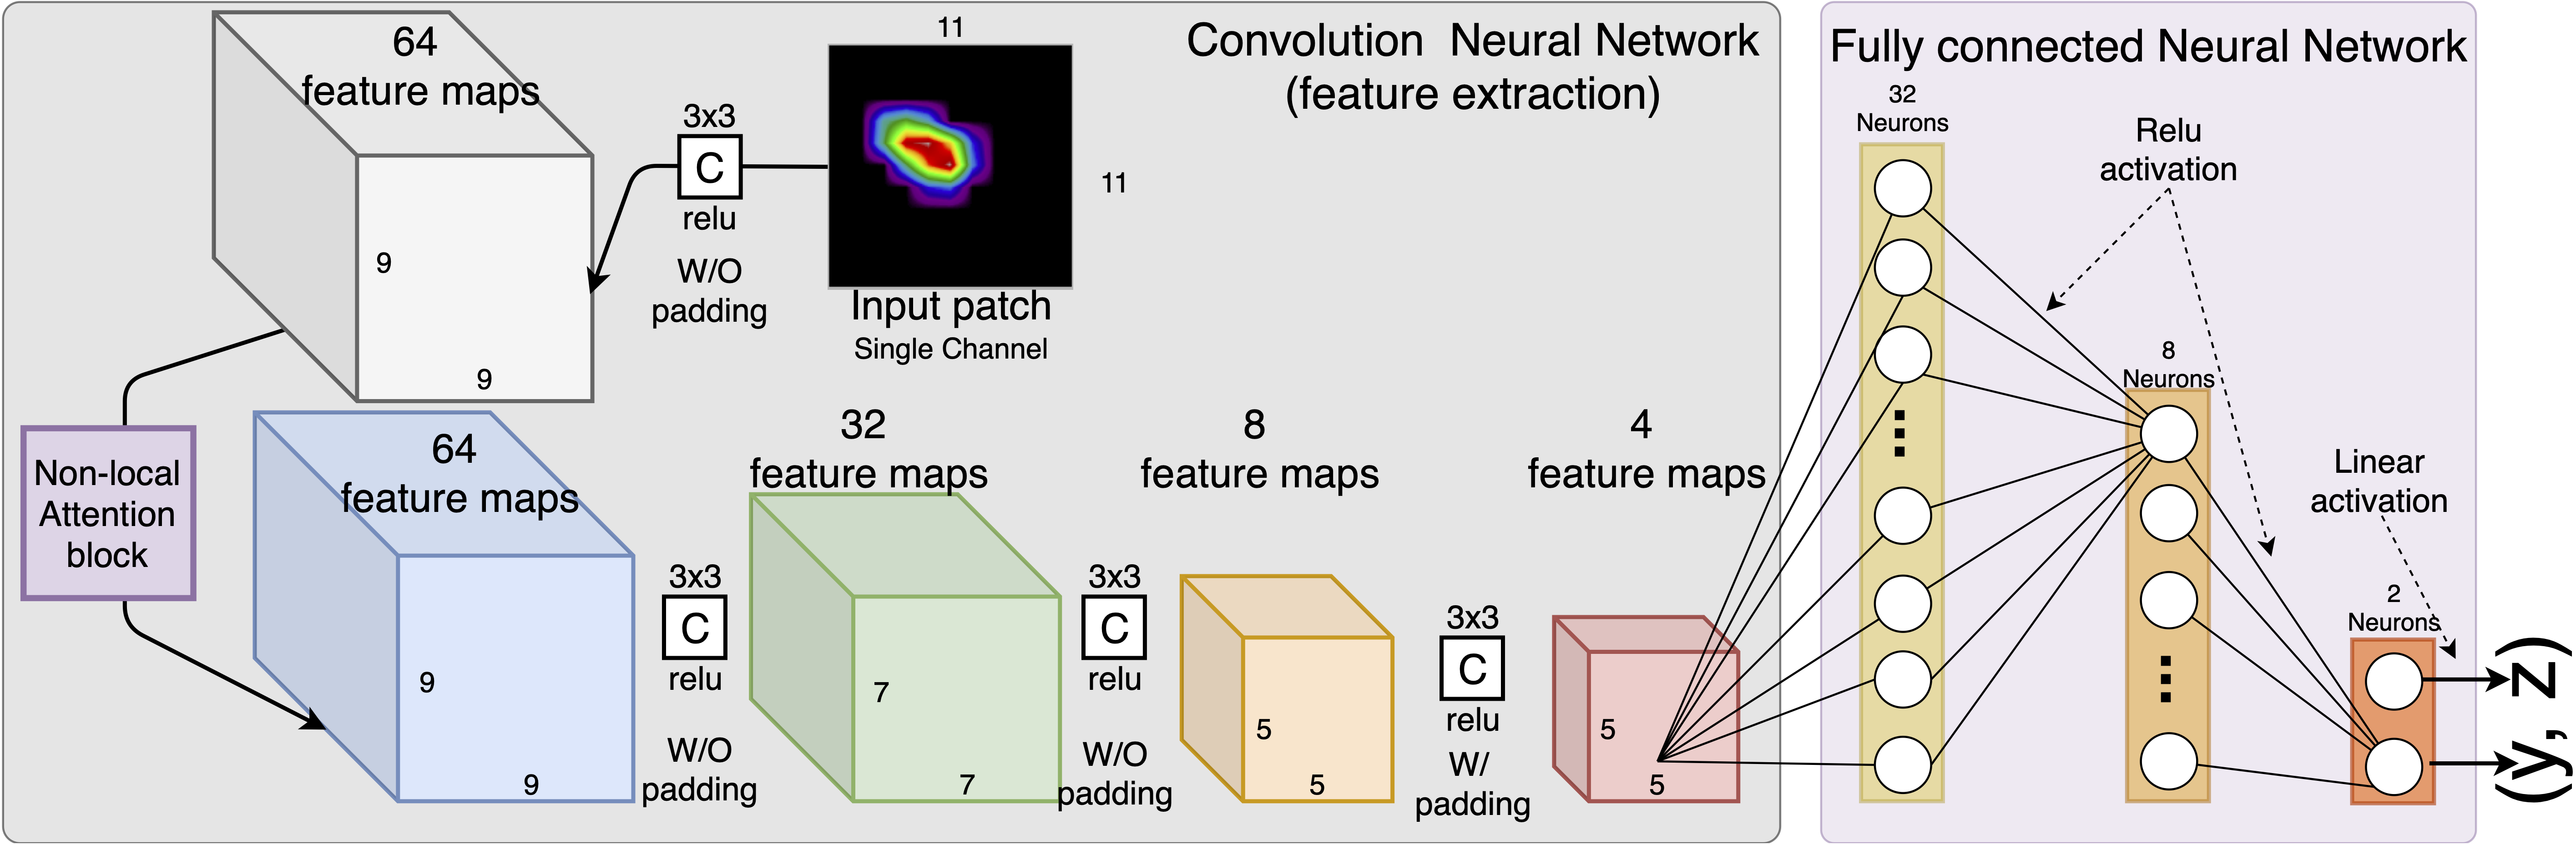
\includegraphics[width=\textwidth]{figures/BraggNN}
	\caption{This is a placeholder.}
\end{figure*}
Lowering from PyTorch to TS IR allows us to perform many useful analyses and transformations on BraggNN that would be extremely difficult or impossible on the original representation; basic optimizations like dead code elimination and constant propagation are supported by TS's graph rewriting functions.
In addition, PyTorch also supports at least two kernel fusion\cite{10.1145/2688500.2688521} tools, proprietary (NNC fuser) and third party (nvfuser).
Such transformations are critical for achieving peak performance on CPUs and hardware accelerators alike but for our purposes, deployment to application specific hardware, we require a broader collection of transformations.
To this end, we turn to a recent addition to the compiler toolchain ecosystem.

\subsection{MLIR}\label{subsec:mlir}

Multi-level Intermediate Representation\cite{https://doi.org/10.48550/arxiv.2002.11054} (MLIR) is a new approach to building reusable and extensible compiler infrastructure.
MLIR is composed of a set of \emph{dialect} IRs, subsets of which are fully mutually compatible outright or by way of translation/legalization.
The various dialects aim to capture and formalize the semantics of compute intensive programs at varying levels of abstraction, as well as namespace related sets of IR transformations/optimizations (called \emph{passes}).
Our entrypoint into this compiler stack is the Torch dialect\cite{torch-mlir}, a high-fidelity mapping from TS IR to MLIR native IR, that provides for us the necessary shape refinement mentioned above, and various other translations that reduce the impedance mismatch between TS and MLIR.

While Torch dialect acts as a thin shim around TS IR and does little "heavy lifting", the same cannot be said for other dialects in MLIR.
For example, the linalg dialect is designed to address the hierarchical optimization problem, wherein the goal is to enable code generation of efficient code or dispatch to existing, previously optimized, kernel code, without sacrificing ease of use and performance for either path.
Practically speaking, this entails representations of common mathematical operations, such as \mintinline{python}{matmul}, \mintinline{python}{conv}, and \mintinline{python}{batchnorm}, explicitly declaring semantics that are traditionally obtained only through compiler analysis (such as memory dependency) and transformations on such operations completely preserving such semantics.
We make extensive use of the linalg dialect as an intermediary between lower-level dialects, such as the affine and structured control flow dialects, and Torch dialect.
The structured control flow dialect is a straightforward formalization of control flow primitives, such as conditionals and loops, so we do not discuss it in great detail.
The affine dialect, on the other hand, provides a formalization of semantics that lend themselves to polyhedral compilation techniques\cite{polyhedral-mlir}, i.e., techniques that make dependence analysis and loop transformations efficient and reliable.

\commnt{possibly this should go into a broken diagram/figure, each of the lowerings}{It's worth working through a small example at this point that intersects all of the levels of translation discussed so far.
	Consider the familiar 2D convolution operation, ubiquitous in so called convolutional neural networks (CNNs), and comprising several of the layers in BraggNN.
	A PyTorch representation of this operation is as straightforward} as
\begin{longlisting}
	\inputminted{python}{sources/conv2d.py}
	\caption[Long Code Example]{A long code example which will break across pages.}
	\label{lst:long}
\end{longlisting}
\noindent where \mintinline{python}{*_channel} parameters specify the multiplicity of the input and output feature maps, \mintinline{python}{kernel_size} refers to the characteristic dimension of the convolution filter/kernel, and \mintinline{python}{padding} refers to the amount of zero padding that should be added to the input.
In terms of abstraction, it's important to note here that this is a completely declarative and abstract description of the operation, with neither specification nor constraint on how the data should be initialized or ordered in memory, nor the hardware that the computation should run on, nor whether some constituent computations could be (or should be) performed in parallel.

The first rung down the ladder of abstraction is TorchScript IR:
\begin{longlisting}
	\inputminted{mlir}{sources/conv2d.ts}
	\caption[Long Code Example]{A long code example which will break across pages.}
	\label{lst:long}
\end{longlisting}
where it's worth pointing out that the tensor corresponding to the weights of the convolution, namely \mintinline{mlir}{%conv1.weight}, has a fully refined type (including data type, shape and striding) but neither the input tensor (\mintinline{mlir}{%x.1}) nor the output tensor (\mintinline{mlir}{%out.1}) do.
This implies that the types of those tensors are determined at runtime, while, as already mentioned, these dimensions are necessary for further lowering.
Thus the input shape needs to be supplied by the user, while the output shape is in principle determined by the implementation of \mintinline{mlir}{aten::conv2d}.
This is reflected in the next rung, the first representation of 2D convolution as MLIR:
\begin{longlisting}
	\inputminted{mlir}{sources/conv2d.torch.mlir}
	\caption[Long Code Example]{A long code example which will break across pages.}
	\label{lst:long}
\end{longlisting}
Note that here we have all types for all values fully refined, as well as having their \commnt{footnote defining}{value semantics} emphasized by the \mintinline{mlir}{vtensor} type.
Aside from type refinement, the Torch dialect performs complex operator decomposition and translation to basic operations, as evident in the lowering to the linalg dialect:
\begin{longlisting}
	\inputminted{mlir}{sources/conv2d.linalg.mlir}
	\caption[Long Code Example]{A long code example which will break across pages.}
	\label{lst:long}
\end{longlisting}
where we observe that \mintinline{mlir}{torch.aten.conv2d} is decomposed into output tensor declaration (\mintinline{mlir}{linalg.init_tensor}), output tensor initialization (\mintinline{mlir}{linalg.fill}) and finally actual convolution (\mintinline{mlir}{linalg.conv_2d_nchw_fchw}).
For a more involved example of this decomposition see the \commnt{appendix softmax}{appendix}.
One important thing to note at this level of abstraction is that the decomposition is as such in the service of preserving value semantics.
While value semantics are important for various analyses, they are in themselves an artifact of abstraction: if we can guarantee no aliasing of \mintinline{mlir}{%arg0} occurs downstream of this convolution, then the \mintinline{mlir}{linalg.init_tensor} and \mintinline{mlir}{linalg.fill} are wasteful (of memory and clock cycles).
More on this in the methodology section.
Note that here we also clearly see, for the first time, the sense in which MLIR is a family of mutually compatible dialects; \mintinline{mlir}{arith.constant} operations are part of the arith dialect, which is mutually compatible with most dialects in MLIR.

From the linalg representation there are two choices for the next level of abstraction:
\begin{enumerate}
	\item Affine Loops (affine dialect);
	\item Structured Control Flow Loops (scf dialect).
\end{enumerate}
Ultimately we will opt for only one of these (scf) but it's edifying to inspect both:
\begin{longlisting}
	\inputminted{mlir}{sources/conv2d.affine.mlir}
	\caption[Long Code Example]{A long code example which will break across pages.}
	\label{lst:long}
\end{longlisting}
Affine maps characterize the affine dialect.
As already mentioned, this dialect is a precise formalization of polyhedral semantics; it's worth emphasizing that syntax such as \mintinline{mlir}{affine_map<(d0, d1) -> (d0 + d1)>} (which represents the projection $y = d0 + d1$) is structured and computable.
That is to say, it has an object representation in memory during compilation that can be manipulated and queried.
For example, this representation is employed in proving the existence or absence of data dependencies between iterations of adjacent loop nests (such as those above) as a prerequisite for loop fusion; this is implemented by constructing the set of constraints on loop indices and memory accesses (i.e., \mintinline{mlir}{%1[%arg1, %arg2, %arg3, %arg4]} and \mintinline{mlir}{%arg0[%arg1, %arg5, %3, %4]}) and computing the feasible region (using either Presburger Arithmetic or \commnt{cite}{Fourier--Motzkin elimination}).
Note that this analysis abides a straightforward implementation exactly due to the explicit inclusion of the affine mapping between the loop iteration space and the memory accesses.
\begin{longlisting}
	\inputminted{mlir}{sources/conv2d.scf.mlir}
	\caption[Long Code Example]{A long code example which will break across pages.}
	\label{lst:long}
\end{longlisting}
The lowering to structured loops illustrates the kinds of insights available from lowering the level of abstraction of an arbitrary DNN operation; while it's certainly straightforward to infer from the mathematical \commnt{maybe write down the equation?}{definition of convolution} that it is "embarrassingly parallel" across dimensions \commnt{double check}{(\mintinline{mlir}{batch_size, output_channels, output_height, output_width}),} this property is manifestly obvious when considering the resulting loop nest; note that in the inner body of the second loop nest, the load and stores from/to the ultimate result of the convolution (\mintinline{mlir}{%2}) only depend on (\mintinline{mlir}{%arg1, %arg2, %arg3, %arg4}) and that the store follows the load.
Thus, it becomes clear from just inspection that the inner loops (on \mintinline{mlir}{%arg5}, \mintinline{mlir}{%arg6}, \mintinline{mlir}{%arg7}) can be fully unrolled and that the resulting single loop can be parallelized across (\mintinline{mlir}{%c1} $\times$ \mintinline{mlir}{%c64} $\times$ \mintinline{mlir}{%c9} $\times$ \mintinline{mlir}{%c9}) workers.

The next step in the lowering is LLVM IR, an IR that is, technically speaking, not an MLIR dialect, even though there does exist an LLVM dialect and we do lower to LLVM dialect as an intermediary between MLIR and LLVM.
The purpose of further lowering to LLVM IR is to produce a representation of BraggNN that high-level synthesis tools can consume.
In particular, Xilinx's Vitis HLS, based on the Autopilot project\cite{Zhang2008}, recently enabled passing LLVM IR to the tool, rather than C/C++.
We Briefly discuss the role of HLS in the translation process.

\subsection{High-Level Synthesis and Down}\label{subsec:hlsdown}

High-level synthesis tools produce RTL descriptions of digital designs from high-level representations, such as C or C++\cite{10.1145/2514740, ferrandi2021bambu}, or in the case of Vitis HLS, LLVM IR.
Given a high-level representation, HLS fundamentally does three things in order to produce a corresponding RTL design:
\begin{enumerate}
	\item HLS schedules operations (such as \mintinline{mlir}{fmult}, \mintinline{mlir}{fadd}, \mintinline{mlir}{load}, \mintinline{mlir}{store}) in order to determine which such operations should occur during each clock-cycle. A schedule depends on three parameters:
	      \begin{itemize}
		      \item The topological ordering of the DFG/CFG (i.e., the dependencies of operations on results of other operations and resources);
		      \item The completion time for each operation;
		      \item The user's desired clock rate/frequency/cycle length.
	      \end{itemize}
	\item HLS associates high-level operations to particular RTL instantiations (called \emph{bindings}) for those operations; for example whether to associate an addition operation followed by a multiplication operation to two separate DSP instances, or whether to associate them both with a single DSP instance configured to compute fused-multiply-add;
	\item HLS builds an FSM that cycles (transitions from state to state) through the sequence of operations in the schedule (and extracts its RTL representation).
\end{enumerate}
In general, the scheduling problem can be expressed as an integer programming problem\cite{tuprints9272}
\begin{figure}[H]
	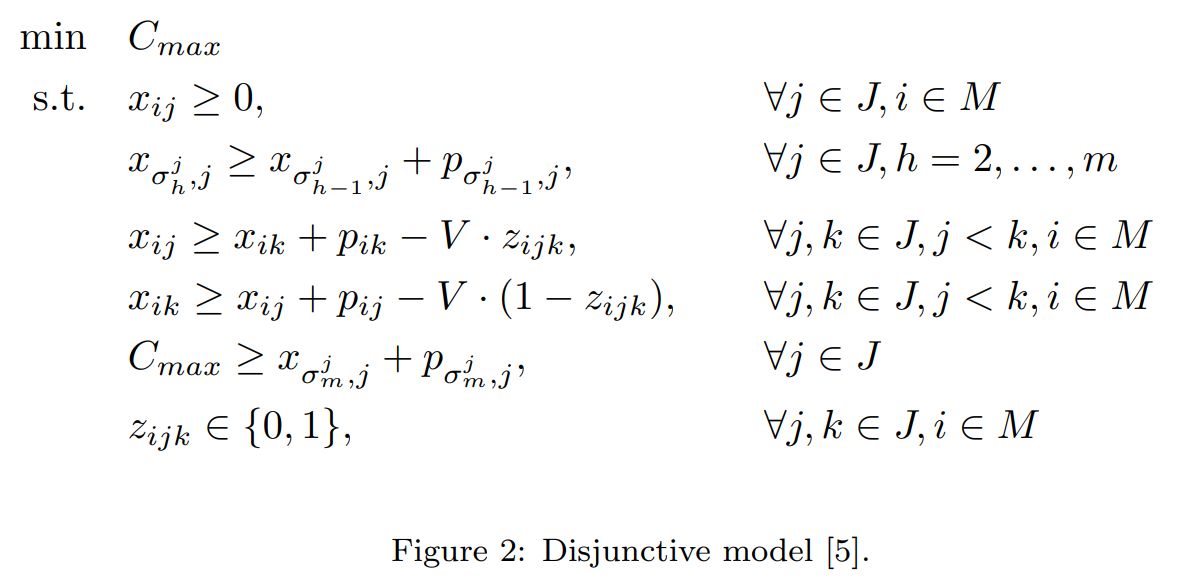
\includegraphics[width=\columnwidth]{figures/schedule}
	\caption{This is a placeholder.}
\end{figure}
whose solution in general, as all for all integer programming problems, is NP-Hard (NP-complete even).
For certain instances, the scheduling problem can be formulated as a system of difference constraints:
\begin{figure}[H]
	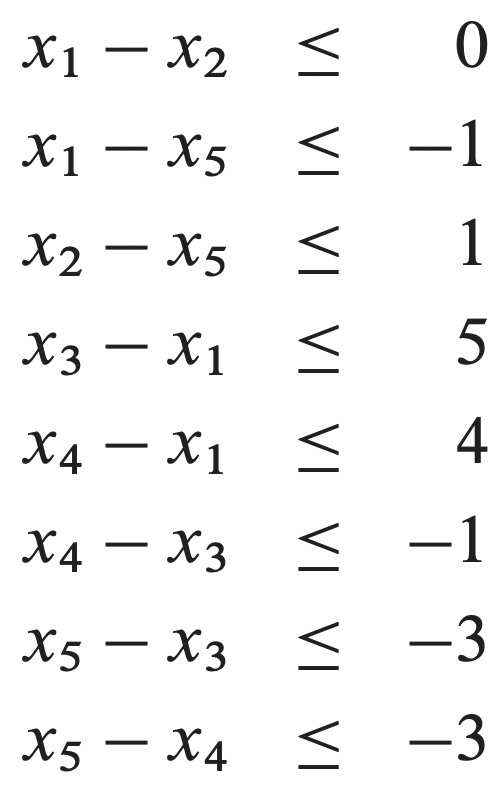
\includegraphics[height=\columnwidth]{figures/sdc_constraints}
	\caption{This is a placeholder.}
\end{figure}
\begin{figure}
	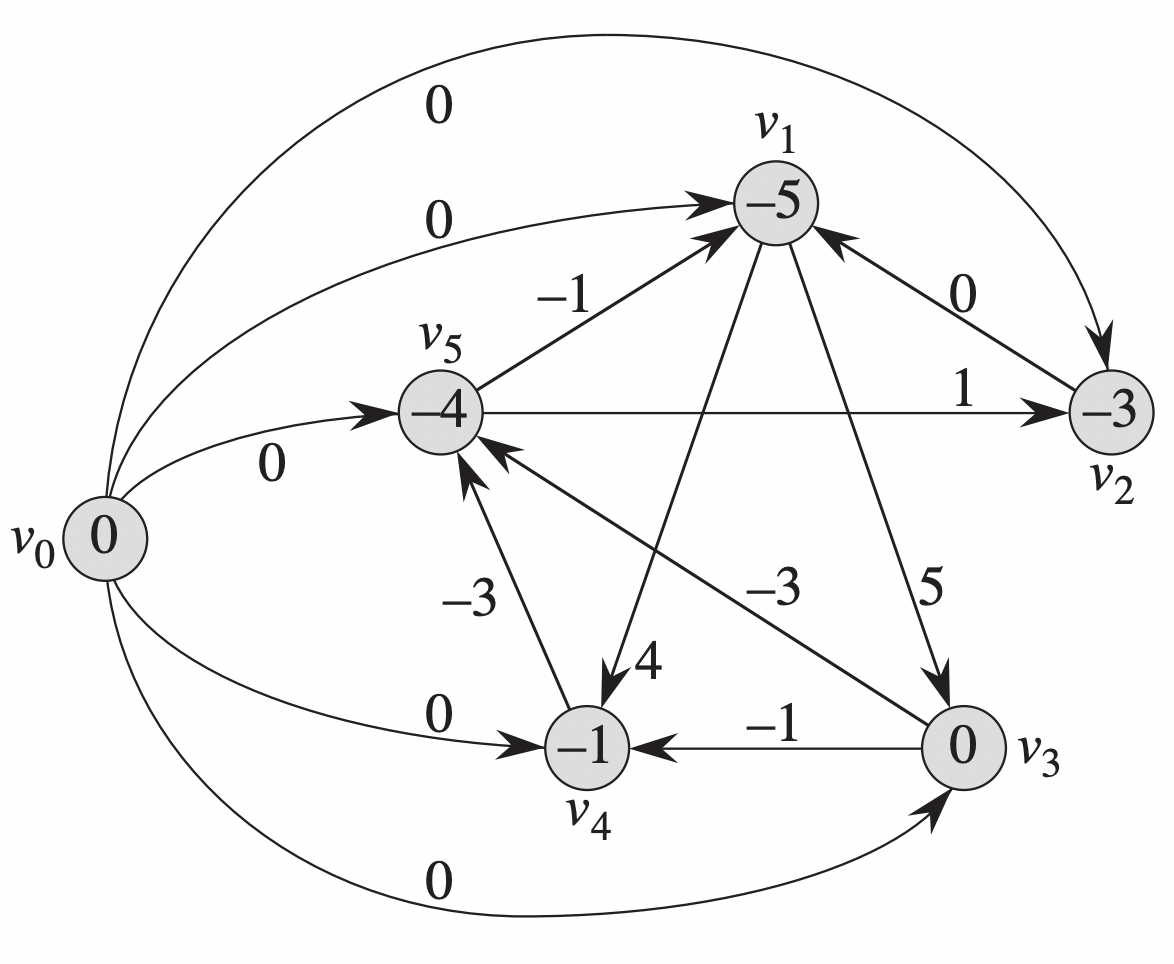
\includegraphics[width=\columnwidth]{figures/sdc_graph}
	\caption{This is a placeholder.}
\end{figure}

Such a formulation induces a unimodular matrix representation of the constraint system
\begin{figure}
	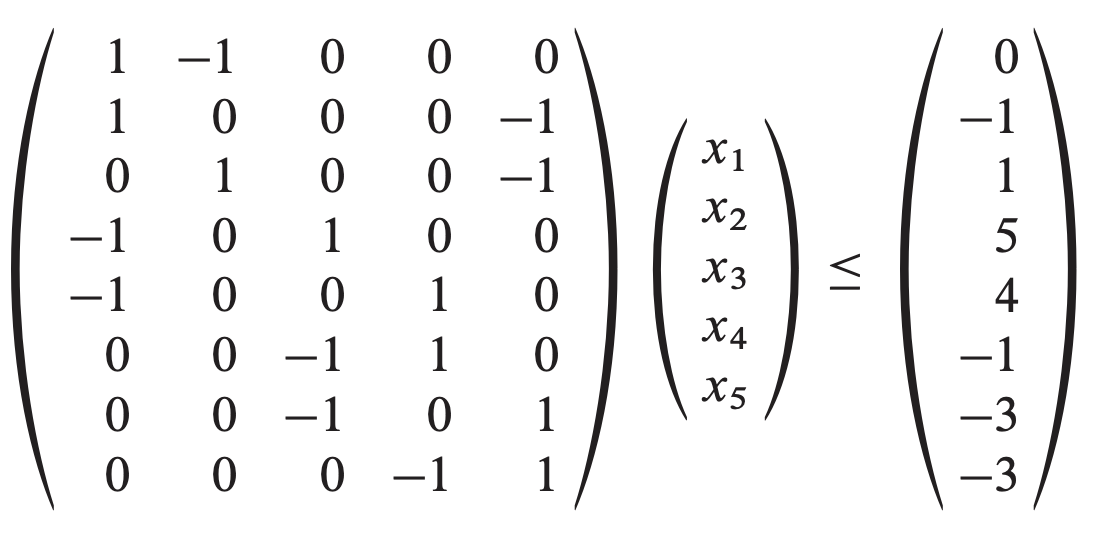
\includegraphics[width=\columnwidth]{figures/unimodular}
	\caption{This is a placeholder.}
\end{figure}
which is amenable to Bellman-Ford $O(n^2 + mn)$\commnt{this is phrased poorly - unimodular guarantees you integral solutions to the LP but also gives you the shortest path analogy property}{ for checking consistency of a solution (essentially the shortest path problem) }and an LP approach for optimizing the critical path\cite{1688836}.

In addition to fulfilling these three fundamental tasks, High-level synthesis tools such as Vitis, Bambu\cite{ferrandi2021bambu}, LegUp\cite{10.1145/2514740} perform standard compiler optimization passes on the IR (that they either receive or produce internally).
Optimization passes such as \commnt{maybe define these? maybe not since i\'ll discuss them in the methodology section}{store-load forwarding, common subexpression elimination, and constant propagation}.
Loop-unrolling and tiling are also performed at the behest of the user.
Ostensibly, after running the LLVM IR corresponding to BraggNN through e.g. Vitis, we should have a RTL description of a digital design that implements the functionality of BraggNN, including control flow, floating point operations (potentially, by way of DSPs), and memory I/O.
At this level of abstraction, there remain two more steps prior to being able to actually deploy to an FPGA; one of them being a final lowering, so called logic synthesis, and the other being Place and Route (PnR).

Logic synthesis is the process of mapping RTL to actual hardware primitives on the FPGA (so called \emph{technology mapping}), such as lookup tables (LUTs), registers, and DSPs (in cases where they haven't been explicitly instantiated).
Logic synthesis produces a network list (netlist) describing the connectivity of various parts of the design.
For example,
\begin{longlisting}
	\inputminted{verilog}{sources/always.v}
	\caption[Long Code Example]{A long code example which will break across pages.}
	\label{lst:long}
\end{longlisting}
\noindent corresponds to a state of an FSM during which the registers \mintinline{verilog}{notlhs17_reg_1608}, \mintinline{verilog}{notrhs18_reg_1613}, \mintinline{verilog}{tmp_8_reg_1618} are updated with new values from wires (\mintinline{verilog}{notlhs17_fu_1076_p2}, \mintinline{verilog}{notrhs18_fu_1082_p2}, \mintinline{verilog}{grp_fu_646_p2}).
Assuming these registers are updated in other states from differing wires, this logic will synthesize to muxs and possibly mux trees (depending on how many different input wires feed these same registers).
Such muxs (and mux trees) are actually implemented using LUTs (more on this in the methodology section).
Another example is the implementation of floating point units in terms of DSPs; depending on user parameters and/or design analysis, DSP resource consumption for floating point multiplication and addition can different greatly (more on this in the methodology section).

Finally, after the netlist has been produced, the entire design undergoes PnR.
The goal of PnR is to determine which configurable logic block within an FPGA should implement each of the units of logic required by the digital design.
PnR algorithms need to minimize distances between related units of functionality (in order to minimize wire delay), balance wire density across the entire fabric of the FPGA (in order to reduce route congestion), and maximize the clock speed of the design (a function of both wire delay, logic complexity, and route congestion).
The final, routed design, can then be deployed to the FPGA by producing a proprietary \emph{bitstream}, which is flashed to the FPGA.

In general, both of these final steps (logic synthesis and PnR) can only be performed by the proprietary tools of the hardware manufacturers (e.g., Vivado by Xilinx) and thus, from our perspective their inner workings are completely unknown.
Recently, open source alternatives for certain FPGAs have become available, thanks to herculean efforts made to reverse engineer the various bitstream formats of, for example, some of Xilinx's architectures\cite{6546003}, and reimplement logic synthesis in open source.
Namely, \cite{wolf2013yosys} is a framework for Verilog RTL synthesis.
It provides a basic set of synthesis algorithms for mapping to Xilinx and Lattice FPGA (as well as ASIC standard cells).
We use Yosys as a basis of comparison for commercial tools and as a way to investigate the limitations of those tools (i.e., when Vivado fails, we can reason by analogy with Yosys, why it might've failed).